\chapter{問題}
\label{issue}
% この研究が解く問題をシャープに記述する

本章では、サービス利用者がインターネットサービスを利用する際に利用規約を読む場面において、本研究の解決する問題について述べる。また、利用規約が読まれないことに対しての問題点や原因を明確化した後に、問題解決のための要件を述べる。

\section{利用規約の状況}
2020年に消費者庁が「デジタル・プラットフォーマーの取引慣行等に関する実態調査」の一環として、デジタル広告分野についての実態調査を行い、検索サービス及びSNSの利用者向け(消費者向け)アンケート調査を行った。この調査の結果を以下に示す。

\begin{figure}[h]
  \begin{center}
      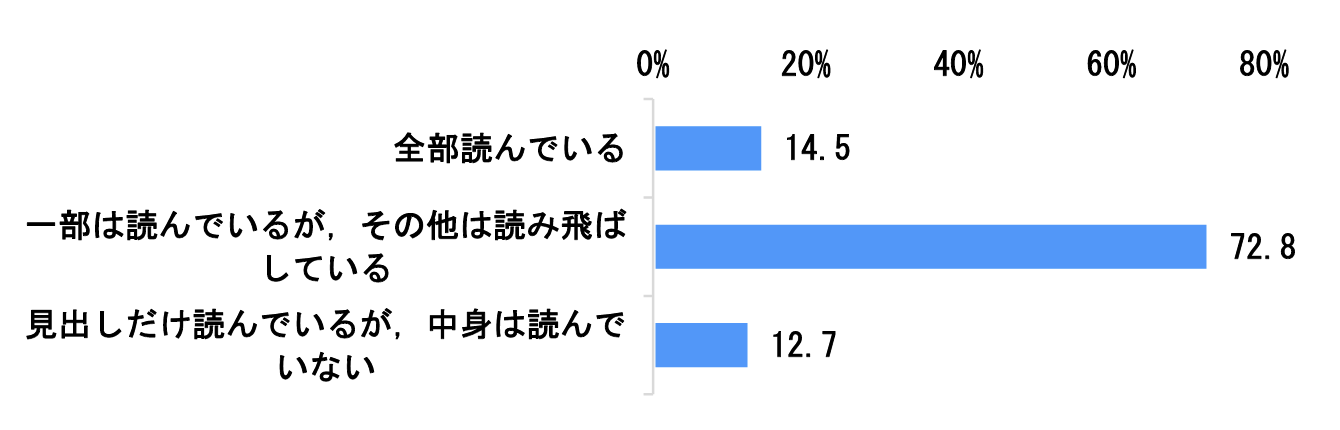
\includegraphics[width=14cm]{img/searchtosyomu.png}
      \caption{検索サービスの利用規約をどの程度読んでいるか(回答数:448)、消費者庁, デジタル・プラットフォーム事業者の取引慣行等に関する実態調査(デジタル広告分野)について(最終報告)\cite{jftc2021} より引用}
      \label{img:searcjtosyomu}
  \end{center}
\end{figure}